\documentclass{article}
\usepackage{tikz}
\usepackage[compat=1.1.0]{tikz-feynhand}
\begin{document}
\[
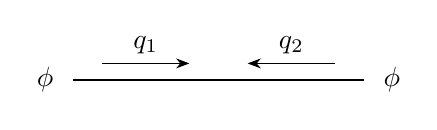
\begin{tikzpicture}[baseline=-0.6ex,scale=1]
  \begin{feynhand}
    \vertex (c) at (0,0);
    \vertex (l) at (-1.85,0);
    \vertex (r) at (1.85,0);
    \vertex[blob] at (0,0);
    \propag[plain,mom={$q_1$}] (l) to (c);
    \propag[plain,mom'={$q_2$}] (r) to (c);
  \end{feynhand}
  \node at ([xshift=-10pt]l) {$\phi$};
  \node at ([xshift=10pt]r) {$\phi$};
\end{tikzpicture}
\]
\end{document}
